\documentclass[a4paper,12pt]{article}
\usepackage{blindtext}
\usepackage[utf8]{inputenc}
\usepackage{graphicx}
\usepackage{enumitem}
\usepackage{booktabs}
\usepackage{verbatim}
\usepackage{makecell}
\usepackage[section]{placeins}
\usepackage{float}

\begin{document}
\begin{center}
	
\includegraphics{Graphics/uplogo.jpg}
	
	{\Huge 
		2017 COS 301 Project \linebreak
		Project Management System \linebreak 
		\par}
	
	{\Huge
		TEAM CODE 9
		\linebreak
		\par}
	
	\begin{LARGE}
		Seonin David
		\linebreak
		\linebreak
		Joshua Moodley
		\linebreak
		\linebreak
		Jaques Smulders
		\linebreak
		\linebreak
		Jordan Daubinet
		\linebreak
		\linebreak
		Nicaedin Suklul
	\end{LARGE}
\end{center}

\begin{figure}[b]
	\centering
	
\includegraphics[width=8cm]{Graphics/kpmgLogo.jpg}
\end{figure}

\newpage
\tableofcontents
\newpage

\newpage
\section{Introduction}
    \subsection{Purpose}
      \begin{flushleft}
        The purpose of this document is to provide a detailed description of the requirements for the Project Management System. It will explain the purpose and features of the system, as well as system constraints. This document is intended to be proposed to University of Pretoria lecturers and the KPMG the project owner, as well as a reference for developing the first version of the project management system.
      \end{flushleft}
 
  \subsection{Scope}
      \begin{flushleft}
        KPMG currently have a web based project management system named EMS which handles allocation and management of assigned projects for all employees and project managers.The current system does not cover the spectrum of requirements that they demand. They require further functionality from the system and they wish to control more business needs and communication through a single portal. The client needs require us to create a new design of their current system and an update of their current interface.
        \linebreak
        \linebreak
        KPMG's project management system will be a web based application that allows for the creation and management of projects. It will handle a notification system for notification requests and notification acknowledgements and and per-user calendar overview to display all current project information currently assigned to that user. For all projects currently administered, the system is also required to display client Location and direction information to the employees assigned to the project.
        \linebreak
        \linebreak
        KPMG's project management system will further require Microsoft Outlook integration in the form of a toolbar to be created for Microsoft Outlook which manages the chain of responsibility for notification requests and notification acknowledgements.
      \end{flushleft}


\section{Overall Description}
\subsection{Product Perspective}
\subsubsection{System interfaces}
TBA
\subsubsection{User interfaces}
A web application will be available for the employee to interact with, as well as a quick response feature that will be provided in Outlook.
\subsubsection{Hardware interfaces}
N/A
\subsubsection{Software interfaces}
Our system will run on a Microsoft environment. 
\subsubsection{Communication Interfaces}
Outlook will be the medium through which the user will interact and receive notifications. The protocols used will be HTTP/S with addition to SMTP/POP3/IMAP. Futhermore, communication will be encapsulated by Outlook's API.
\subsubsection{Memory}
For our system we will be using a MongoDB cluster, that will be hosted on a NodeJS server.

\newpage
\subsection{Constraints}
	\begin{itemize}
		\item The project must be completed in the given time frame with progress on        track with demo expectations.
		\item The project must not utilize technologies with require cost resources.
		\item The project must utilize Microsoft Outlook as a communication interface       for sending and confirming requests
		\item The project must be run as a local host and not deployed on a company         server
	\end{itemize}
\subsection{Assumption and Dependencies}


\section{Specific Requirements}
	\subsection{Functional Requirements}
		\subsubsection{FR1: Employee Functions}
			\begin{itemize}
				\item \textbf{FR1.1}: An employee will be able to log in to their account on the system
				\item \textbf{FR1.2}: An employee will be able to create their own profile with their        respective skills and previous work experience
				\item \textbf{FR1.3}: An employees will receive a notification when they are assigned to a    newly created project 
				
				\item \textbf{FR1.4}: An Employee must be able to to view their currently assigned           project and view their past completed projects that where assigned        to them on their profile. 
				
				\item \textbf{FR1.5}: An employee will be able to add personal or other events to the        calendar their calender, that do not clash with any existing               projects they are currently assigned to. If a newly created event        does clash, an error will be displayed.  
				
				\item \textbf{FR1.6}: When an employee clicks on a project in the calendar, it will show     all the project details and a map of the clients location should be       displayed as well as directions to the client.
				
				\item \textbf{FR1.7}: An employees will not be able to remove a project that is assigned     to them from their calender.
				
				\item \textbf{FR1.8}: Employees should confirm wheather they have attended training or not, this will be conformed with trainer.
			\end{itemize}
	
	\subsubsection{FR2: Manager functions}
	\begin{itemize}
		\item \textbf{FR2.1}: A manager will be able to log in and create a project.
		
		\item \textbf{FR2.2}: A manager will be able to assign system recommended employees to a      newly created projects
		
		\item \textbf{FR2.3}: A manager will be able change employees if the manager is unhappy with     the recommendation by the system, pending director approval.
		
		\item \textbf{FR2.4}: A manager will be allowed to remove a project from the system, pending director approval
		
		\item \textbf{FR2.5}: A project manager will be able to view all projects that they are managing
	\end{itemize}
	
	\subsubsection{FR3: System Functions}
	\begin{itemize}
		\item \textbf{FR3.1}: The system will assign employees to a project based
		on their skill level and past project experience. 
		
		\item \textbf{FR3.2}: The system will find all the employees that have the required skills     for the job and give it to the manager as a recommendation.
		
		\item \textbf{FR3.3}: The system will only select employees if they are not already           assigned to a project.
		
		\item \textbf{FR3.4}: Employee data with skills and past work experience
		will be entered on the system and updated after each project. 
		
		\item \textbf{FR3.5}: System will reassign another employee, pending 
		approval, if an employee takes leave during the project.
		
		\item \textbf{FR3.6}: Every employee that is assigned to a project will get
		the full project duration and details on their calendar. 
		
		\item \textbf{FR3.7}: The system should be able to provide the location of and direction      to the client to all employees assigned to the respective project
		
		\item \textbf{FR3.8}:The system will preload all employees training dates
		at the beginning of the year. 
		
		
		\item \textbf{FR3.9}: The system will preload all employees training dates at the beginning of the year.
	\end{itemize}
	

\subsection{Non Functional Requirements}
 \begin{itemize}
	\item Color Scheme - There will have to be a pleasing colour scheme for           the system, one that represents the colours of KPMG
	
	\item Security - The system will have to cater for employee and client            security, There will have to be measures put into place to prevent         the database and server falling prey to malicious attacks.
	 
	\item Performance - The system will have to manage many users at the same         time, mostly based on the number of employees stationed at the            Pretoria branch
	
	\item Concurrency - The system will have to support multiple users at the         same time
	
	\item Scalability - The system will have to be able to adapt to a larger          environment and expand beyond its normal scope of function
\end{itemize}
	
\subsection{Architectural Requirements}

\begin{paragraph}
        The system will be designed using the n-tier architecture (Specifically 3-tier), where the system is divided into three layers}
        \begin{itemize}
            \item 1. Presentation Layer
            \item 2. Application Layer
            \item 3. Data Layer
        \end{itemize}
         Each layer will be modifiable without having to change the entire application. As a result of the aforementioned, maintenance and adding extra functionality is easier. Overall complexity of code over all layers will be reduced thus making the layers reusable in other applications.By using this architecture system will allow the different members in our teams to modify different layers without interference. It is possible to deploy each layer (Specifically the data and application layers) over multiple different locations for better reliability and performance.
\end{paragraph}
 
  
  \subsubsection{Presentation Layer}
    \begin{paragraph}
       This is the layer the user will be interacting with. It encompasses the actual apps (Android, iOS and web), and any interactions that the users have with them.     
    \end{paragraph}
    \textbf{The presentation layer include:  }
      \begin{itemize}
        \item What to display and when to display it, it’s the logic behind the webpages and the control between access from one to another.
      \end{itemize}
  
  \subsubsection{Application Layer}
    \begin{paragraph}
        The application layer contains all the business logic of the system - it makes logical decisions based on the interactions from the presentation layer and the data from the data layer.    
    \end{paragraph}

    \textbf{The decisions made by this layer include:}
          \begin{itemize}
            \item Allow admin users to be able to add/ remove client projects and assign these to employees who will be working on these projects.
            \item Automatically update calendars of the employees.
            \item Crosscheck projects before assigning projects to an employee.
            \item Server communication over the internet.
            \item Scheduling Assistant calculations. 
            \item Limit an employee from being able to edit the projects that have been prepopulated.
            \item Allow an employee  to add other events to his/ her calendar if these do not clash with the prepopulated events.
            \item Session management.
          \end{itemize}
  
  \subsubsection{Data Layer}
    \textbf{The data layer is where the data and information used by the application layer is stored. This information includes:}
    \begin{itemize}
        \item Recommended time slots where all employees are available. 
        \item Server storage with mongodb
        \item View individual employee calendar and assigned projects. 
    \end{itemize}
    
\section{Use Case Diagrams}
	\subsection{Assigning Projects}
	\includegraphics[width=15cm,height=20cm]{Functional_Use_Cases/Assigning_Projects.jpg}
	\subsection{Managing Projects}
	\includegraphics[width=15cm,height=20cm]{Functional_Use_Cases/Managing_Projects.jpg}
	\subsection{Veiw Projects}
	\includegraphics[width=15cm,height=20cm]{Functional_Use_Cases/View_Projects.jpg}
	\subsection{Training}
	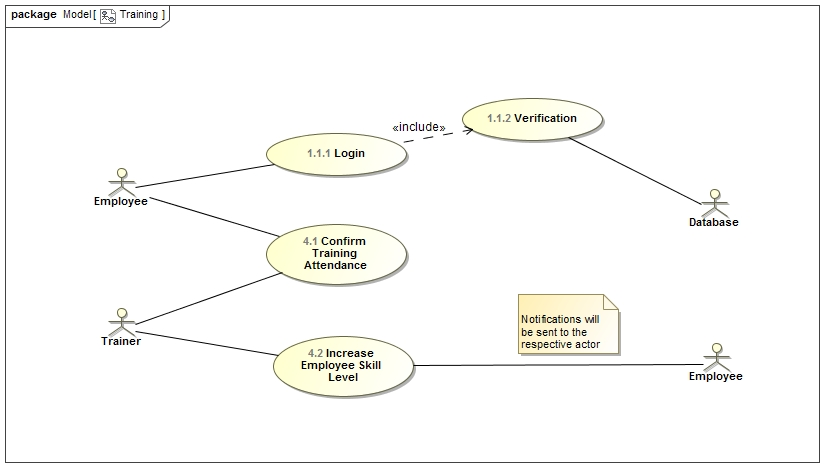
\includegraphics[width=15cm,height=15cm]{Functional_Use_Cases/Training.jpg}
	
\section{Deployment Diagram}
\includegraphics[width=15cm,height=15cm]{Graphics/KPMG.jpg}

\newpage

\section{Tracibility Matrix}
\begin{table}[]
\centering
\caption{Tracibility Matrix}
\label{my-label}
\resizebox{1.2\textwidth}{!}{%
\begin{tabular}{|l|c|c|c|c|c|c|c|c|c|c|c|c|c|c|c|c|}
\hline
       & \multicolumn{1}{l|}{Priority} & \multicolumn{1}{l|}{UC 1.1} & \multicolumn{1}{l|}{UC 1.2} & \multicolumn{1}{l|}{UC 1.3} & \multicolumn{1}{l|}{UC 1.4} & \multicolumn{1}{l|}{UC 1.5} & \multicolumn{1}{l|}{UC 2.1} & \multicolumn{1}{l|}{UC 2.2} & \multicolumn{1}{l|}{UC 2.3} & \multicolumn{1}{l|}{UC 2.4} & \multicolumn{1}{l|}{UC 3.1} & \multicolumn{1}{l|}{UC 3.2} & \multicolumn{1}{l|}{UC 3.3} & \multicolumn{1}{l|}{UC 3.4} & \multicolumn{1}{l|}{UC 4.1} & \multicolumn{1}{l|}{UC 4.2} \\ \hline
FR 1   &                               &                             &                             &                             &                             &                             &                             &                             &                             &                             &                             &                             &                             &                             &                             &                             \\ \hline
FR 1.1 & 2                             & X                           &                             &                             &                             &                             &                             &                             &                             &                             &                             &                             &                             &                             &                             &                             \\
FR 1.2 & 1                             &                             &                             &                             &                             &                             &                             &                             &                             &                             & X                           &                             &                             &                             &                             &                             \\
FR 1.4 & 3                             &                             &                             &                             &                             &                             &                             &                             &                             &                             &                             & X                           &                             &                             &                             &                             \\ \hline
FR 2   &                               &                             &                             &                             &                             &                             &                             &                             &                             &                             &                             &                             &                             &                             &                             &                             \\ \hline
FR 2.1 & 2                             & X                           &                             &                             &                             &                             &                             &                             &                             &                             &                             &                             &                             &                             &                             &                             \\
FR 2.2 & 3                             &                             & X                           &                             &                             &                             &                             &                             &                             &                             &                             &                             &                             &                             &                             &                             \\
FR 2.3 & 1                             &                             &                             &                             &                             &                             &                             & X                           &                             &                             &                             &                             &                             &                             &                             &                             \\ \hline
FR 3   &                               &                             &                             &                             &                             &                             &                             &                             &                             &                             &                             &                             &                             &                             &                             &                             \\ \hline
FR 3.1 & 4                             &                             &                             &                             & X                           &                             &                             &                             &                             &                             &                             &                             &                             &                             &                             &                             \\
FR 3.2 & 1                             &                             &                             & X                           &                             &                             &                             &                             &                             &                             &                             &                             & X                           &                             &                             &                             \\
FR 3.3 & 5                             &                             &                             & X                           &                             &                             &                             &                             &                             &                             &                             &                             & X                           &                             &                             &                             \\
FR 3.4 & 6                             &                             &                             & X                           &                             &                             &                             &                             &                             &                             &                             &                             & X                           &                             &                             &                             \\
FR 3.5 & 2                             &                             &                             &                             &                             &                             & X                           &                             &                             &                             &                             &                             &                             &                             &                             &                             \\
FR 3.6 & 3                             &                             &                             &                             &                             &                             &                             &                             &                             &                             &                             & X                           &                             &                             &                             &                             \\
FR 3.8 & 7                             &                             &                             &                             &                             &                             &                             &                             &                             &                             &                             &                             &                             &                             & X                           &                            
\end{tabular}%
}
\end{table}
\end{document}
